% Input from reports/phase2/ with amsmath,
% graphicx and cite loaded. Numbers come from scripts/choose_rul_cap.py
% (results/metrics/fd001_rul_cap_*.{json,csv}); figures from
% notebooks/phase2/05_rul_cap.ipynb. Cites Phase 1 keys in reports/phase1/refs.bib.

\subsection{Choosing the RUL Cap}
\label{sec:target}

A training engine in C-MAPSS runs until failure~\cite{Saxena2008damage},
so its uncapped RUL early in life can exceed 300 cycles. While the engine is
healthy its sensors are flat, so an engine with 300 cycles left cannot be told
apart from one with 200. The usual remedy is a piecewise-linear target,
$\min(y_{u,t},c)$, which is flat at a cap $c$ and then falls to
zero~\cite{Heimes2008recurrent}. Phase~1 used $c=125$ from the literature.
Here the cap is chosen with a rule that opens only \texttt{train\_FD001.txt}.

\paragraph{Health index and onset.}
Inside each training fold, the sensors retained by the variance check and
correlated with the cycles to failure ($|r|\geq0.1$; 15 on FD001) are
z-scored with the fold's statistics. Each one is multiplied by the sign of
that correlation, so that all of them rise toward failure, and the results
are averaged into one health index $h_{u,t}$. For every engine a hinge
\begin{equation}
 h_{u,t}\approx a_u+b_u\max(t-\tau_u,0),\qquad b_u>0,
\end{equation}
is fitted by least squares over every candidate bend $\tau_u$ that leaves at
least five cycles on each side. The onset RUL is $T_u-\tau_u$, where $T_u$ is
the failure cycle. On FD001 it has a median of 92 cycles and ranges from 59 to
180 (Fig.~\ref{fig:target_hinge}).

\paragraph{Selection metric.}
$K$ is the 90th percentile of the onset RULs in the training fold. A
candidate cap is scored on held-out engines by
\begin{equation}
 \mathrm{RMSE}_{\leq K}=\sqrt{\frac{1}{|S|}\sum_{(u,t)\in S}(\hat y_{u,t}-y_{u,t})^2},
\end{equation}
with $S=\{(u,t):y_{u,t}\leq K\}$ the held-out cycles at or below $K$, where $y$ is the true, uncapped RUL. Cycles above $K$ are dropped because, for
nine engines in ten, no degradation is visible there yet, and the official
test engines (cut off before failure) rarely reach those values. Scoring
every held-out cycle would instead prefer no cap, because a capped model
necessarily misses training cycles with RUL above 200
(Table~\ref{tab:target_caps}). The metric is \texttt{rul.data.target.selection\_rmse}
and is shared by all later tuning and ablations.

\paragraph{Results.}
Five split seeds (3 engine-grouped folds each) gave $K$ between 123 and
137 (mean 130). The seed-42 folds give 134, 132 and 123, which matches the
prototype. Random Forest, XGBoost~\cite{Chen2016xgboost} and Elastic
Net~\cite{Zou2005regularization} were retrained with the Phase~1 engineered
features and hyperparameters at caps of 100, 125, 150 and none.
Caps of 150 and none are clearly worse on $\mathrm{RMSE}_{\leq K}$, by 2.5 to
15 cycles. Caps of 100 and 125 are close. Random Forest picks 125 on all five
seeds and XGBoost on four of five (by 0.04 cycles), while Elastic Net picks 100 on all five.
Averaged over the three models, the two caps tie (16.38 vs.\ 16.40).

\begin{table}[t]
\centering
\caption{FD001 held-out RMSE by training cap (mean $\pm$ s.d.\ over five seeds of
the 3-fold mean). ``All'': every held-out cycle. ``$\leq K$'': the selection metric.}
\label{tab:target_caps}
\footnotesize
\setlength{\tabcolsep}{2.5pt}
\begin{tabular}{lcccc}
\hline
Model, metric & 100 & 125 & 150 & none \\
\hline
RF, all & 58.33$\pm$0.21 & 47.94$\pm$0.09 & 41.22$\pm$0.24 & \textbf{36.73}$\pm$0.55 \\
RF, $\leq K$ & 15.62$\pm$0.36 & \textbf{14.97}$\pm$0.30 & 17.42$\pm$0.36 & 23.57$\pm$0.70 \\
XGB, $\leq K$ & 15.57$\pm$0.38 & \textbf{15.54}$\pm$0.38 & 18.19$\pm$0.26 & 24.97$\pm$0.89 \\
EN, $\leq K$ & \textbf{17.94}$\pm$0.14 & 18.68$\pm$0.18 & 22.87$\pm$0.31 & 32.69$\pm$0.73 \\
\hline
\end{tabular}
\end{table}

\paragraph{Sensitivity.}
The choice between 100 and 125 depends on the percentile. With the 85th
percentile or lower ($K\leq117$), all 15 seed--model runs pick 100. With the
95th ($K\approx141$), all 15 pick 125. The 90th percentile lies on the
boundary (9 of 15 runs pick 125). This agrees with the prototype, where
$K\approx106$ selected 100.

\paragraph{Decision and caveats.}
The rule rules out 150 and an uncapped target, but it cannot separate 100
from 125. We keep $c=125$. The strongest Phase~1 model prefers it on every
seed, and the other Phase~2 results already use it, so switching would cost a
full retrain for no measurable gain. Four caveats apply. (i)~The official test
RMSE at $c=125$ (16.21) was known before this rule was designed, so this
section shows that 125 is defensible from training data alone; it is not a
blind choice. (ii)~Only the tabular models were rerun; the sequence models
may prefer a different cap. (iii)~Hyperparameters were not retuned per cap.
(iv)~The hinge assumes a single bend, and noisy engines can stretch the
upper tail of the onset distribution, which is where $K$ is read.

\begin{figure}[t]
\centering
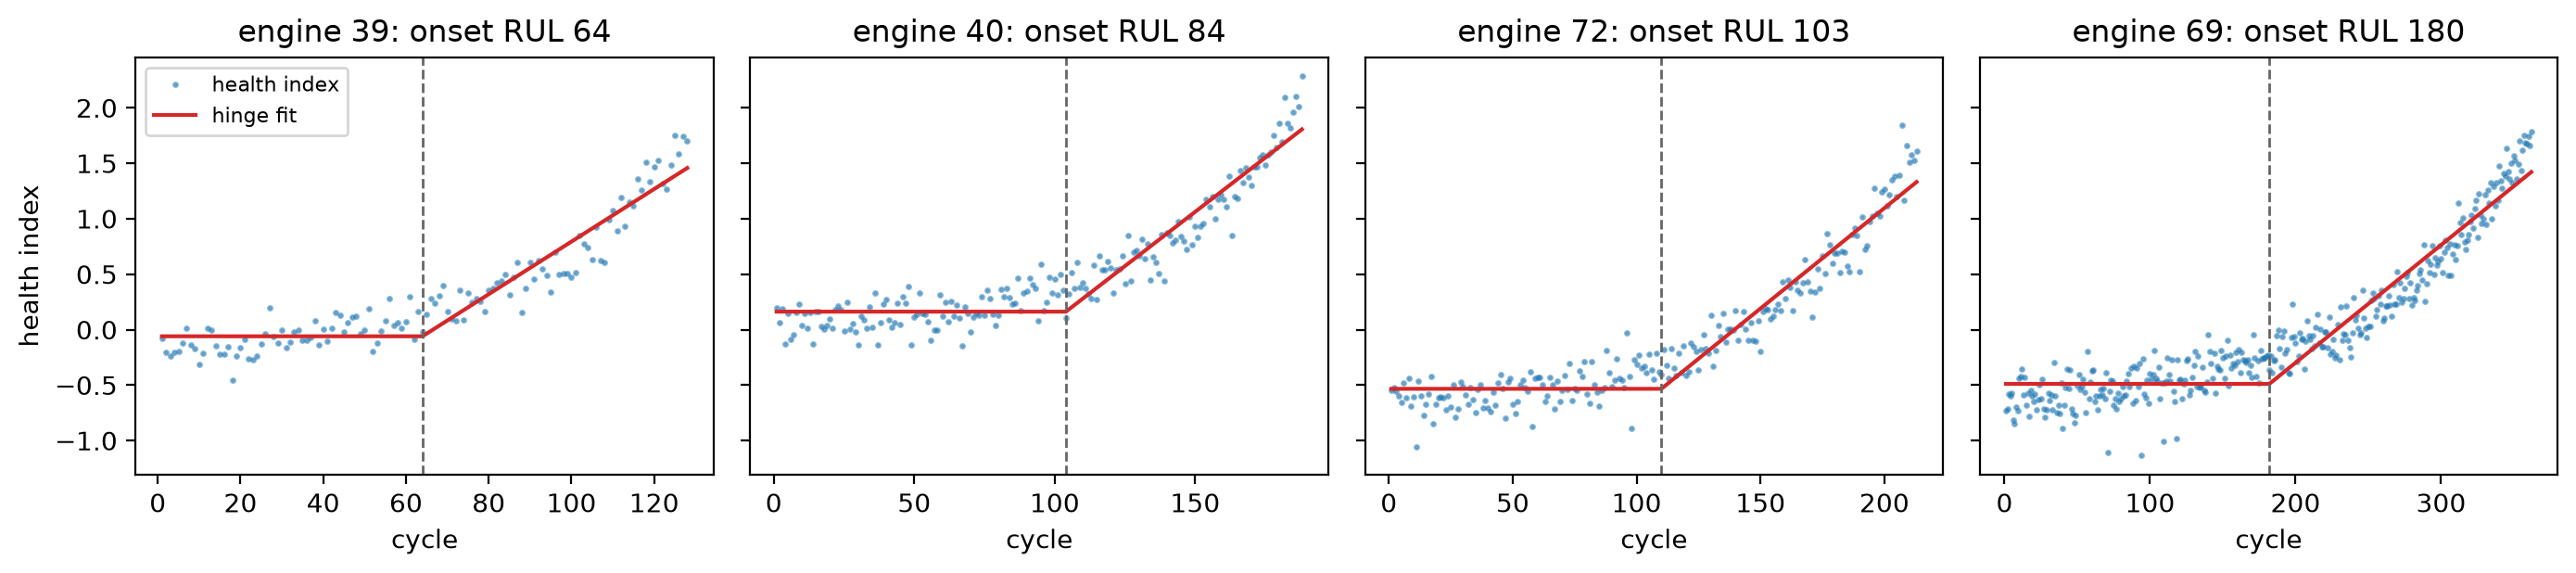
\includegraphics[width=\linewidth]{../../results/figures/fd001_rul_cap_hinge_fits.png}\\[2pt]
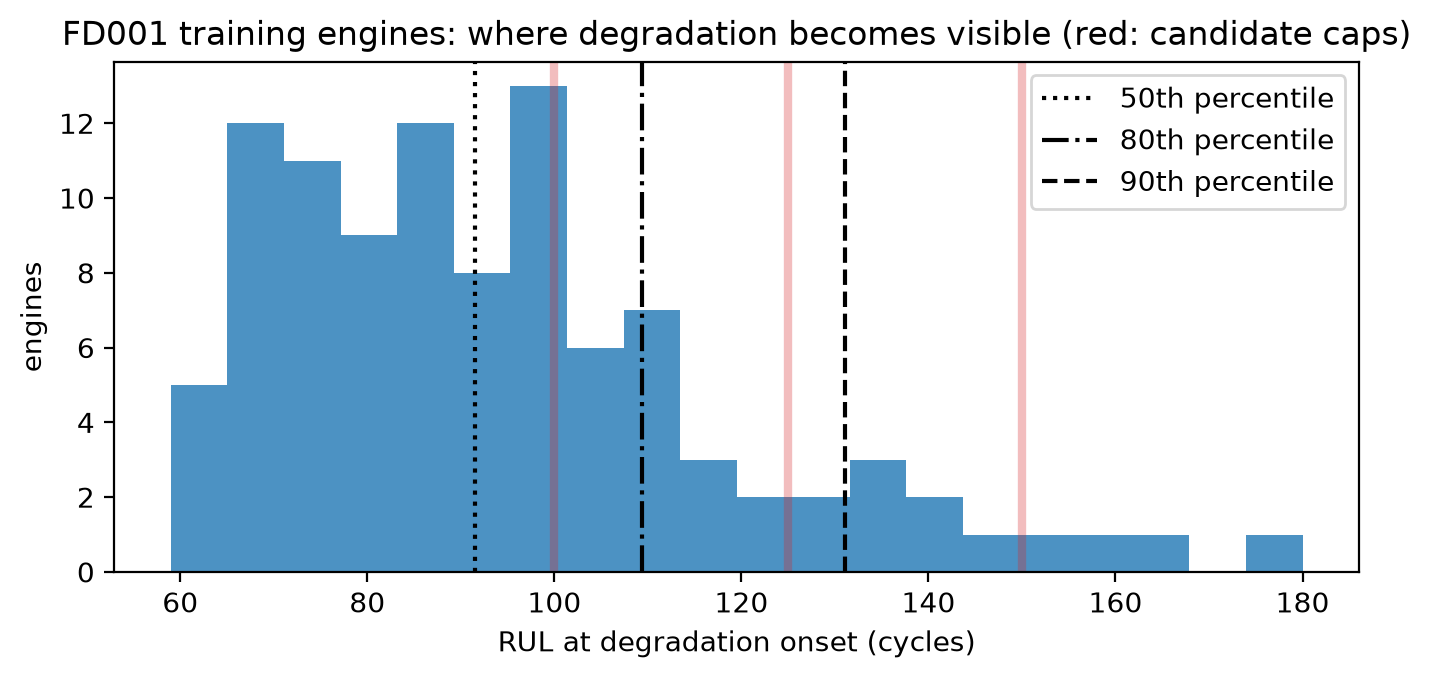
\includegraphics[width=0.49\linewidth]{../../results/figures/fd001_rul_cap_onset_distribution.png}\hfill
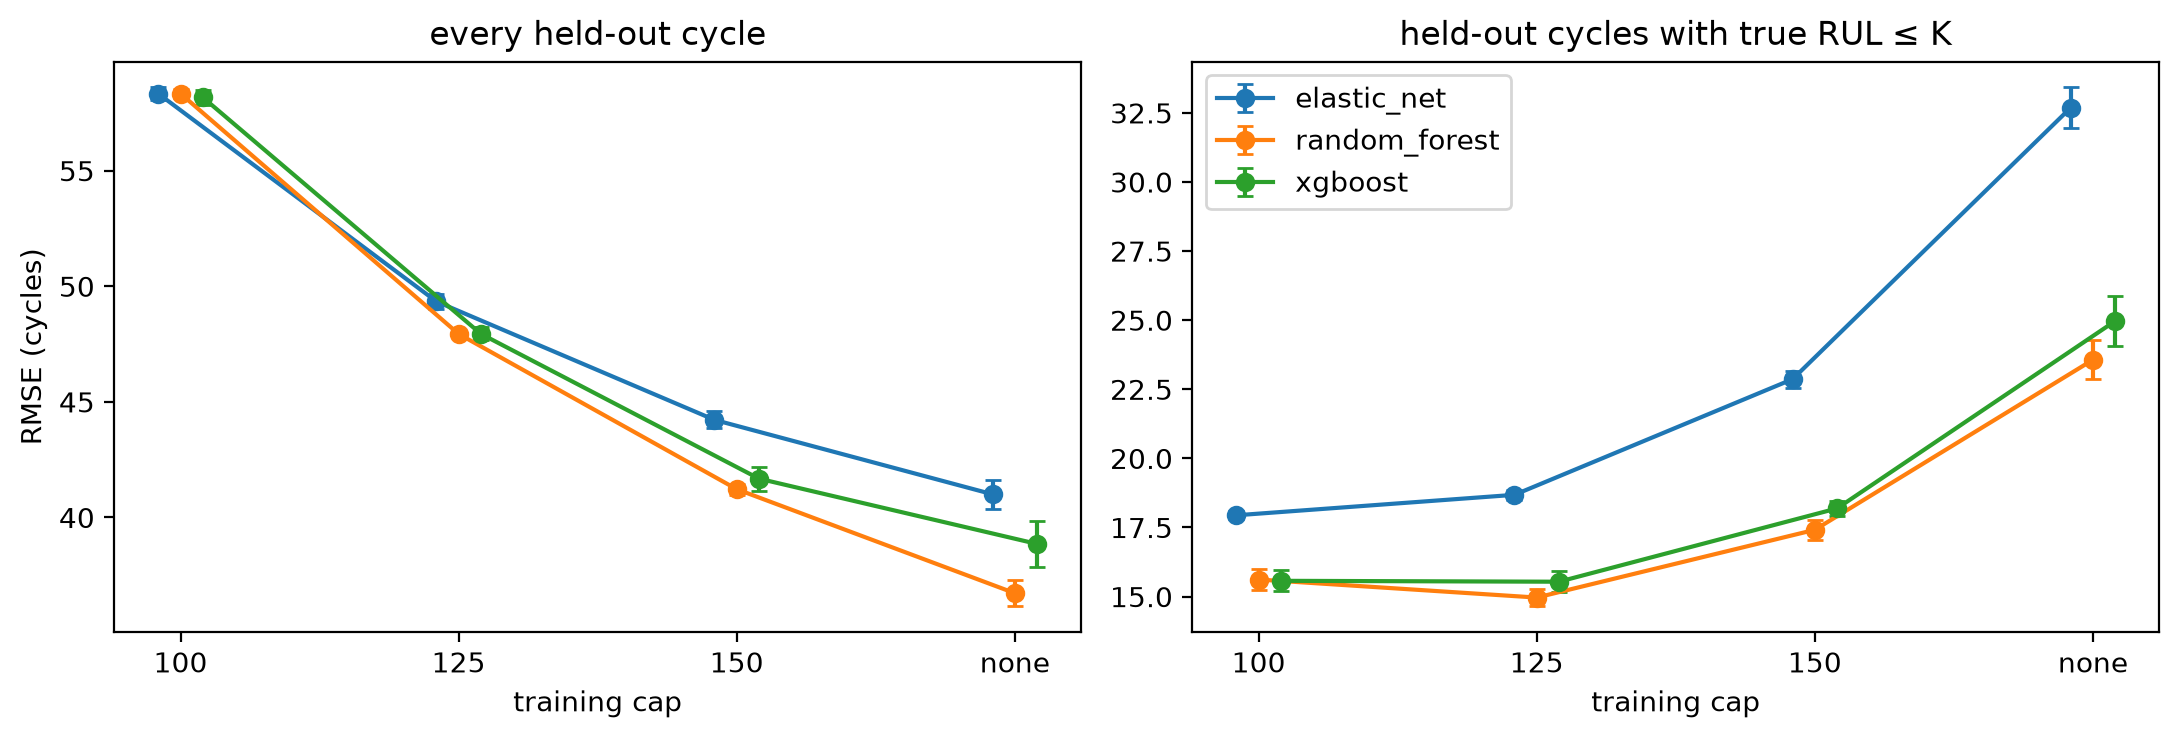
\includegraphics[width=0.49\linewidth]{../../results/figures/fd001_rul_cap_score_by_cap.png}
\caption{Top: hinge fits for four FD001 training engines. Bottom left: onset RUL
distribution, with candidate caps in red. Bottom right: held-out RMSE by cap,
on every cycle and on cycles with true RUL $\leq K$.}
\label{fig:target_hinge}
\end{figure}
